% Autor: Lukas Deeken
% Letzte Bearbeitung: 01.05.2022

\chapter{Elektromechanische Systeme}

\section{Akkumulator}

\subsection{Zellenauswahl}

Wichtig bei der zellenauswahl ist das stets jede individuelle zelle für sich begutachtet werden muss. es gibt bei den diversen Bauformen und chemischen Zusammensetzungen gewissen Tendenzen welche im folgen erläutert werden. Jedoch ist die Überlappung dieser Eigenschaften in der Regel so groß das sich augenscheinlich vollkommen unterschiedliche Zellen für einen ähnlichen Einsatzzweck eignen.

\subsubsection{Vergleich der Speicherarten}

%im nachfolgenden wird die zuerst die Energie berechnet die ein klassiches Formula Studentfahrzeug bei einem typischen bremsvorgang freisetzt und damit die enrgie die mann mindestens speichern können müsste um mit der speciherform auf sinnvolle art und weise eine rekuperation umszusetzten. Im anschluss wird diese energie in eine ungefähre masse an speicherelementen umgesetzt um zu zeigen inwiefern sich diese form der enrgiespeicherung für den einsatz eignet. im nachfolgenden wird die masse an speciherelementen bestimmt um 6 Kwh energie zu speichern da dies der typsiche energieverbrauch eines formula student fahrzueuges im Endurance ist. dieser wert wurde im rahmen eines benchmarkings mit den fahrzeuigen anderer teams über die letzten jahre 2016 bis 2019 errechnet.

Im folgenden errechnen wir die Energie welche bei einem durchschnittlich Bremsvorghang eines formula student fahrzeuges aufgenommen werden müsste. 

\begin{equation}
\glsc{symb:E_kin} = \dfrac{1}{2} * \glsc{symb:m} * \glsc{symb:v}^2
\end{equation}

\glsc{symb:m} = 220Kg
\\
\glsc{symb:v}\textsubscript{Start} = 30m/s
\\
\glsc{symb:v}\textsubscript{end} = 5m/s
\\
\glsc{symb:E_kin} * \glsc{symb:mu} = 74,8kJ
\\

Physikalische Speicher (Kondensatoren)
\\
	Kondensatoren erreichen ein sehr hohes Leistungsgewicht, zeichnen sich jedoch durch eine geringe Energiedichte aus, sowohl gravimetrisch als auch volumetrisch. daher eignet sich diese Form der Energiespeicherung nur um kurzfristige transienten zu glätten aber nicht um gar ganze Bremsvorgänge an Energie zu speichern.\\
	Der Kondensator mit der höchsten energiedicht welcher bei Würth Elektronik verfügbar ist erreicht 3600J/Kg. Somit würde man ca. 20Kg dieser Kondensatoren brauchen um damit effektiv rekuperieren zu können. Bei einem Gewicht für die akuzellen alleine im TY22 von ca. 30,7Kg ergibt sich das der superkondensator nach akltuellem stand keine sinnvoll einsetzbare technologie darstellt.
\\
Thermische Speicher (Salzakkumulator)
\\
	sind im rahmen der formula student verboten Stand 2022, daher wird hier nicht weiter auf diese form des energiespeichers eingegangen
\\
Mechanische Speicher (Schwungrad)
\\
	Zeichnung sich durch relativ gute energiedichte als auch leistungdichte aus und bilden damit wahrscheinlich am ehesten eine realistische form des kurfristigen speichers für ein formula student fahrzeug. Jedoch sind solche systeme sehr komplex sowohl mechanisch, elektrisch als auch regelungstechnisch im vergleich zu den anderen systemen. Die lagerung und sichere unterbringung des schwungrades in einem formel fahrzeug birgt große technische herausforderungen
\\
Chemische Speicher (Klassische Akkuzelle)
\\
	Der typische im Rahmen der formula studnet von allen teams eingesetzte energiespeicher. In der verfügbaren bandbreite findet man so ziemlich das optimum an leistungs als auch energiedichte.

\subsubsection{Runde vs Pouch vs Prismatische Zellen}
%tabelle
(
	Puch zelle

in der regelung höhere packungsdichte möglich damit höherte volumetrische enrgie und lkeistungsdichte
in der regel weniger zellen weniger als 300 manschmal sogar nur 150
weiches gehäuse ist leicht zu beschädigen, bedarf vorischtiger umgang 
aufblähen beim laden und entladen muss bei konstruktion berücksichtigt werden sonst platzenb der zellen möglich


Rundzelle

geringere fertigungstoleranzen durch serienfertigung idr kein matching erforderlich
hoher grad an standardisierung damit folgen mechanische austauschbarkeit und gute marktverfügbarkeit
Hartes gehäuse damit geringe wahrscheinlichkeit von penetrastion durch spitze objekte
bedarf in der regel sehr vieler zellen 600 und mehr, daher hohe mechanische komplexität

Prismatische Zellen

vorgefertigtes paket aus rund oder pouchzellen
sehr wenige zellen kleiner 150
sehr geringe mechanische komplexität da das paket in der regel mit elektrischen und mechanischen anbindungspunkten kommt meist sind auch schon temperatur sensoren integriert
meist jedoch sehr schwer aufgrund der ausrichtung auf industrielle bedürfnisse


Im rahmen des TY22 haben wir uns für den einsatz von rundzellen entschieden da diese nach unserem kenntnisstand gravimetrisch die höchste energiedichte liefern wir uns langfristig auf ein konzept festelgen wollten und so bei einsatz einer neuen akkuztelle nur gerinfügige änderungen an dem akku machen müssen sofern das 18650 format weiterhin populär bleibt. Außerdem war dies im rahmen der lieferschwierigkeiten im bereich der akuzellen im jahr 2021 die beste option um tatsächlich auch an akkuzellen für den bau des fahrzeuges zu kommen
)

\subsubsection{Zellchemie und Rekuperation}

Im folgenden eine tabellarische gegenüberstellung von \acfirst{LiFePo4} zellen und \acfirst{Li-ion} Zellen. Diese Tabelle basiert auf einer Sichtung von mehr als 30 verschiedenen Akkuzellen welche im rahmen des Projektes auf ihre Eignung für den Einsatz im Fahrzeug geprüft wurden. Liion umfasst dabei ein konglomerat aus diversen zellchemien welches eigentlich auch lifepo4 mit einschließt. Zur vereinfachung des vergleiches wurden alle liion chemieen mit einem typ. arbeitsbereich von 3-4,2 hierunter zusammengafasst. Die hierbei aufgrund der hohen löeistungsdichte am häufigsten vertretene Chemie ist LiNiMnCoO2



In der analyse ergibt sich das bild das sich \acfirst{LiFePo4} zellen für ein konzept mit hohem rekupoerationsanteil aber niederiger gesamtkapazität eignet während sich liion zellen für ein konzepot mit niedrigerem rekuperationsanteil und hoher gesamtkapazität eignen. Weiterhin muss hier berücksichtigt werden das Lifepo4 zellen meist ein niederigers temperaturmlimit beim laden als beim entladen haben was im betrieb zu einem vorzeitigen ausfall der rekuperation durch zu hohe akkutemperaturen führten kann. daher ist das temperatur managment hier von besoinderer bedeutung.

Das konzept mit hohen rekuströmen ist nur beim AWD Fahrzeug sinvoll anwendbar da hier auch die gesamte bremsenergie, abzüglich der verlsute im antriebsstran und einiger spitzenlasten welche die mechanische bremsanlage abfangen muss, verfügbar ist. Aufgrund der hohen komplexität des AWD systemes wurde beim TY22 auf ein 2WD System gesetzt. Daher ist der einsatz von konkret LiNiMnCoO2 zellen am ehesten sinvoll.

\subsubsection{Temperaturmodell der Zelle}

Auf Basis der Masterarbeit Experimentelle Untersuchung von Batteriesystemen im simulierten niedrigen Erdorbit von Agnes Klein an der Universität Stuttgart konnte ich ein simples thermisches modell der akkuzelle in einer excel tabelle ersytellen. Bei dieser arbeit wurde unter anderem die akkuzellen des types VTC6 innerhalb einer thermnal vakuum kammer betrieben und die thermischen paramter der zelle ermittelt. In folgender Grafik finden sie die dabei ermittelten parameter.

\begin{figure}
	\centering
	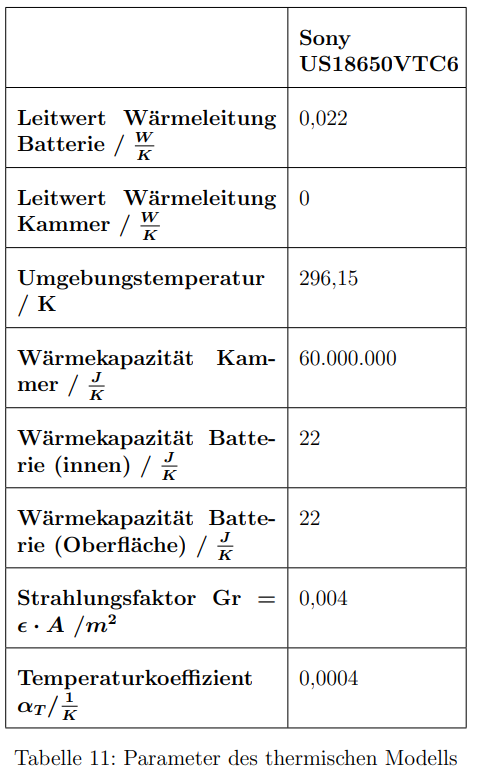
\includegraphics[width=0.4\linewidth]{bilder/Parameter_thermisches_modell_VTC6}
	\caption{}
	\label{fig:parameterthermischesmodellvtc6}
\end{figure}


Damit ergibt sich folgendes Modell.

\begin{equation}
	\glsc{symb:T_celli+1} = (\glsc{symb:I_cell}^2 * \glsc{symb:R_cell} - \glsc{symb:G_th} * (\glsc{symb:T_celli} - \glsc{symb:T_u}) - \glsc{symb:G_r} * \glsc{symb:SBoltz} * (\glsc{symb:T_celli} - \glsc{symb:T_u})^4) * \dfrac{1}{\glsc{symb:C_B} * \glsc{symb:m_Cell}} + \glsc{symb:T_celli}
\end{equation}

Mit diesem Modell ergeben sich folgende Kurvenverläufe für eine Auswahl Entladeströmen

\begin{figure}
	\centering
	\includegraphics[width=0.7\linewidth]{bilder/temperatur_über_energie_vtc6_thermo_modell}
	\caption{}
	\label{fig:temperaturuberenergievtc6thermomodell}
\end{figure}

Mithilfe der folgenden Grafik von der Universität BRNO (MATEC Web of Conferences 313, 00045 (2020)) können wir einen Plausibilitätscheck durchführen. Wir haben hier Messdaten von der Sony VTC6. hierbei sind jedoch die Testbedingungen unbekannt. Als grobe Abschätzung sollte dies jedoch ausreichen

\begin{figure}
	\centering
	\includegraphics[width=0.7\linewidth]{"bilder/Messdaten_VTC6_ temperatur kapazität spannung"}
	\caption{}
	\label{fig:messdatenvtc6-temperatur-kapazitat-spannung}
\end{figure}

Wir sehen das das erstellte modell für den 10A graph um ca. 3°C abweicht. Weiterhin sehen wir das bei der 20A linie die 90°C ca. 0,5Ah früher erreichen. Diese Abweichungen nicht insignifikant, zeigen jedoch das unser modell eher zu hohe als zu niedrige temperaturen ausgiebt was für die zuverlässigkeit des fahrzeuges positiv ist da eine auslegung der kühlung mit diesem modell wahrscheinlich zu einer überkühlung und damit zu einem zu hohen gewicht des kühlsystemes führt was für das erste fahrzeug kein sonderliches problemn darstellt. Die abweichung dürfte darauf zurückzuführen sein das die modellparameter im vakkum ermittelt worden und insofern wärmeübertragung durch konvektion etc. nicht berücksichttigt werden konnte. Um diesem sachverhgalt weiter auf die gründe zu gehen wurde im anschluss eine Simulation mit ansys fluent durchgeführt.

\begin{figure}
	\centering
	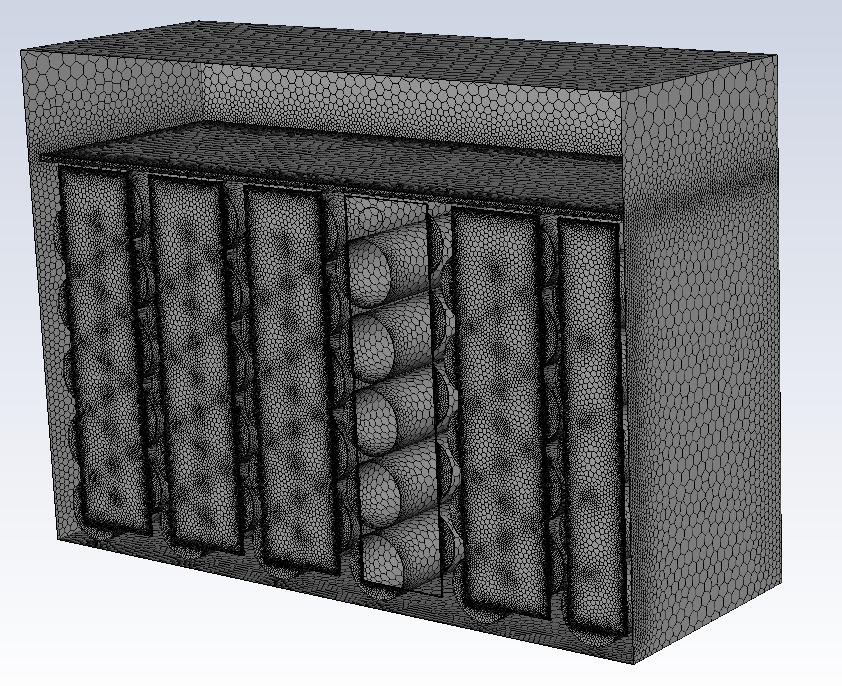
\includegraphics[width=0.7\linewidth]{bilder/Accu_Sim_therm_7_2A_45min_simple_mesh}
	\caption{}
	\label{fig:accusimtherm72a45minsimplemesh}
\end{figure}

\begin{figure}
	\centering
	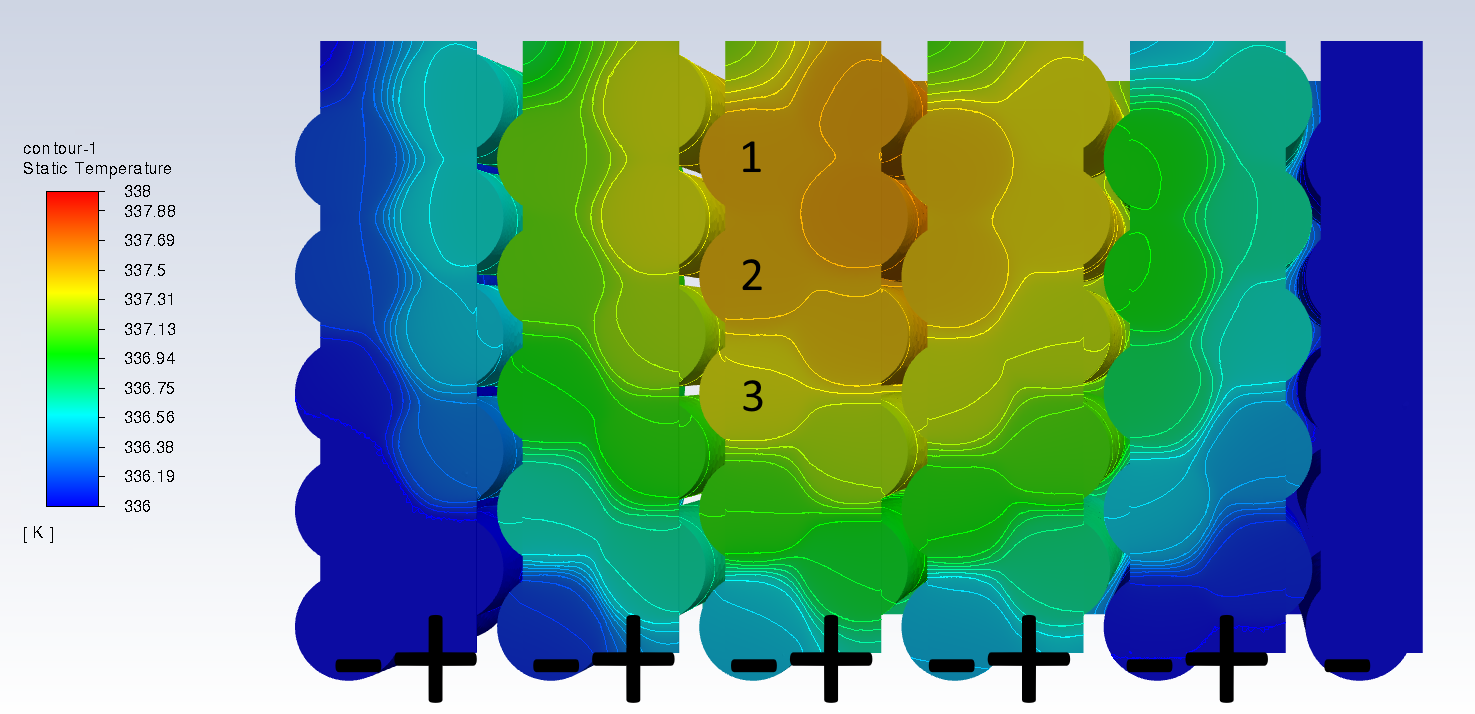
\includegraphics[width=0.7\linewidth]{bilder/Accu_Sim_therm_7_2A_45min_simple}
	\caption{}
	\label{fig:accusimtherm72a45minsimple}
\end{figure}

In dieser simulationb wurde ein gesamter akkustack in seinem gehäuse simuliert. dabei wurde mit einem konstanten strom von 7,2A simuliert. Dieser strom ergibt sich aus der rundenzeitsimulation siehe sectrion. Die Simulation wurde für 32min laufen gelassen um eine gesamtes endurance darzustellen. Ziel der simuzlation ist es die effekte der konvektion zu berücksichtigen aber auch zu sehen in wiefern sich die zellen gegenseitig beeinflussen. Allerdings wurden auch diverse vereinfachungen getroffen insofern das die akkuzellen sich uniform aufwäremn. In der realität dürfte man am negativen pol der akuzelle eine deutlich höhere temperatur feststellen könne als auf der positiven seite. weiterhin wurden diverse teile wie die elektrische isolierung etc. weggelassen da dies den simulations aufwand sonst erheblich vergrößert hätte und die simulation so schon 2 tage benötigt hat. zur analyse, wir sehen nach der simulationszeiot eine hot spot temperature von 64,85°C und eine niedrigste temperatur von 62,85°C. In dieser hinsicht stimmt die ansys simulation eher mit der 10A kurve aus unserem modell zusammen als mit den messdaten. Zusammengefasst stellt man fest das definitiv weitere arbeit in diesem themenbereich von nöten wäre um zu einer optimalen lösung zu kommen dies jedoch aufgrund des engen zeitplanes und des enoremn anderweitigen aufwandes nicht möglich ist.

\subsubsection{Die \glqq Ideale\grqq Akkuzelle}

\section{Elektromotor}
Im großen und ganzen gibt es für die Auswahl des Elektromotors 4 verschiedene in der Formula Student allgemein anerkannte Lösungen. Diese werden nachfolgend erläutert.

\subsection{Emrax}
Beim Emrax Motor handelt es sich um eine Axial Flux Permanent erregte synchron Maschine PMSM. zusammenfassend sind die emrax motoren sehr flacj haben aber einen großen durchmesser. Sie zeichnen sich durch ein hohes drehmoment und damit verhältnismäßig niedrige drehzahlen aus, im bereich von 7-8K RPM. Sie sind nur in recht großen formaten und damit großen leistungen erhältlich so das ein 1 oder 2 motoren antriebskonzept realisierbar ist. Außerdem handelt es sich hierbei um eine reine kauflösung. 

\subsection{AMK}
Die AMK motoren sind radial flux PMSM. Sie sind insofern eher lang und haben kleine druchmesser. Die bauform gleicht insofern eher dem klassischen elektromotor. Sie zeichnen sich durch extrem hohge drehzahlen aus, oberhalb der 20k und damit durch eine enorme leistungsdichte. Sie sind in eher kleinen leistungsdichten zu bekommen so das beinahe nur ein Allrad antrieb sinnvoll umsetzbar ist. Auch hierbei handelt es sich um eine reine kauflösung. 

\subsection{Fischer}
Die Motoren von fischer sind im großen und ganzen gleichzusetzten mit den amk motoren. der große unterschied ist das hier das gehäuse selbst designt werden muss und alle teile selber gefertigt werden müssen. Die stellt große herausfordferungen die fertigungstechnik da es sich dabei auch um 5 achs gefräst6e titanteile handelt. 

\subsection{Selbstbau}
Der selsbtbau ist quais die nächste entwicklungsstufe nach dem fischer motor. Num gilt es nicht nur den motor selber zu fertigung sondern auch die gesamte vorauslegung zu machen. es gibt nur wenige teams die einen selbstbau wagen, und noch werniger die es erfolgreich umsetzten.

\subsection{Entscheidungsfindung}

Die Entscheidung ist an diesem Punkt sehr einfach. Im rahmen dieser projektabreit entsteht der erste e antrioerb aus dem hause baltic racing. damit kommen enrom viele große heruasforderung. das heißt man sollte entweder die einfachste oder die nächst einfachste Lösung nehmen um am ende zu dem ziel des fahrenden autos zu kommen. Und da sich nur der emrax motor effektic für einen zwei rad antrieb eignet ist es der emrax motor gewotrden.

\section{Wechselrichter}
Der wechselrichter wird benötigt um den motor sauber anzusteuern. Ziel ist es aus gleichstrom aus dem akku einen Frequenz und amplituden regelbaren strom zu erzuegen mit dem der motor kontrolliert werden kann. Hier gibt es auch wieder diverse hersteller die im folgenden verglichen werden sollen


!!!Tabelle!!!





\section{Kabelbaum}

\subsection{Kabeldimensionierung}

\subsection{Sicherungsauslegung}

\subsection{Steckverbinder Auswahl}

\subsection{HVD}

\subsection{AIR}

\section{Shutdowncircuit}

\section{Ladesystem / Handcart}

